\documentclass[10pt,a4paper]{article}

% ============================================================
% SHIELD-RAG — Atlantis Press / Springer Nature AISR Format
% ============================================================
\usepackage[utf8]{inputenc}
\usepackage[T1]{fontenc}
\usepackage{mathptmx}
\usepackage[margin=2.5cm,top=3cm]{geometry}
\usepackage{graphicx}
\usepackage{amsmath,amssymb,amsthm}
\usepackage{booktabs}
\usepackage{multirow}
\usepackage{array}
\usepackage[hidelinks]{hyperref}
\usepackage{enumitem}
\usepackage{titlesec}
\usepackage{abstract}
\usepackage{authblk}
\usepackage{caption}

\titleformat{\section}{\normalfont\bfseries\fontsize{11pt}{13pt}\selectfont}{\thesection.}{0.5em}{\MakeUppercase}
\titleformat{\subsection}{\normalfont\bfseries\itshape\fontsize{10pt}{12pt}\selectfont}{\thesubsection.}{0.5em}{}
\titlespacing*{\section}{0pt}{12pt}{6pt}
\titlespacing*{\subsection}{0pt}{10pt}{4pt}

\renewcommand{\abstractnamefont}{\normalfont\bfseries\fontsize{10pt}{12pt}\selectfont}
\renewcommand{\abstracttextfont}{\normalfont\fontsize{10pt}{12pt}\selectfont}
\setlength{\absleftindent}{0cm}
\setlength{\absrightindent}{0cm}

\newtheorem{theorem}{Theorem}
\newtheorem{definition}{Definition}

\captionsetup{font=small,labelfont=bf}

\title{\bfseries\fontsize{14pt}{16pt}\selectfont SHIELD-RAG: A Verified, Subspace-Isolated, and Revocable Privacy-Preserving Framework for Retrieval-Augmented Generation}

\author[1]{First Author\thanks{Corresponding author. Email: first.author@example.edu}}
\author[2]{Second Author}
\affil[1]{Department of Computer Science and Engineering, University Name, City, Country}
\affil[2]{Department of Computer Science and Engineering, University Name, City, Country}
\date{}

\begin{document}
\maketitle

\begin{abstract}
\noindent Retrieval-Augmented Generation (RAG) systems outsource sensitive corpora to semi-trusted cloud infrastructure, exposing them to embedding inversion, knowledge corruption, access-control failures, and post-generation leakage. Prior functional-encryption-based defenses such as CipheRAG lack dynamic user revocation, proven multi-tenant subspace isolation, and formal indistinguishability guarantees for the access gate. We present \textbf{SHIELD-RAG}, a privacy-preserving RAG framework built around three verified mechanisms: (i) an $O(1)$ revocable clearance gateway requiring zero corpus re-encryption; (ii) QR-factorization-based multi-tenant subspace non-interference with a formal proof of exact zero cross-tenant leakage; and (iii) an IND-CPA indistinguishability reduction of the sensitivity-embedded access gate to the Decisional Composite Residuosity (DCR) assumption. We describe the system architecture, threat model, and mathematical formulation of each mechanism, and detail an empirical evaluation on Wikipedia and Natural Questions benchmarks against unaugmented Ada-IPFE, Permission-Aware RAG, and synthetic baselines across scales up to 50,000 documents.
\end{abstract}

\noindent\textbf{Keywords:} Retrieval-Augmented Generation, Functional Encryption, Access Control, Multi-Tenant Isolation, Privacy-Preserving Machine Learning

\vspace{0.5em}

% =========================================================================
\section{Introduction}
\label{sec:intro}

Retrieval-Augmented Generation (RAG) has emerged as an indispensable architecture for enhancing Large Language Models (LLMs) by coupling parametric language representations with non-parametric external knowledge repositories \cite{lewis2020rag}. By retrieving contextually relevant evidence passages at query time, RAG mitigates hallucinations, bridges domain-specific knowledge gaps, and enables seamless data updates without costly model retraining \cite{shuster2021retrieval, khan2025evidencebot}. Consequently, RAG systems are widely adopted across security-critical enterprise sectors, including clinical diagnostic support, proprietary financial intelligence, and legal document discovery \cite{jeong2025permissionaware}.

Despite these functional advantages, outsourcing private corpora to semi-trusted cloud infrastructure introduces severe data privacy and security vulnerabilities across all three RAG processing stages. At the \textbf{retrieval stage}, dense vector embeddings are susceptible to transferable embedding-inversion attacks that reconstruct sensitive text with high fidelity \cite{zhou2026cipherag}, and adversaries can execute black-box knowledge-corruption attacks (e.g., PoisonedRAG \cite{zou2025poisonedrag}) by injecting adversarial passages into the retrieval database. At the \textbf{access-control layer}, conventional enterprise deployments rely on plaintext Identity and Access Management (IAM) metadata filtering \cite{jeong2025permissionaware}; manual policy merging across heterogeneous models (RBAC/ABAC) leads to privilege escalation, and shared multi-tenant vector indices risk unintended cross-tenant similarity leakage unless mathematical non-interference is enforced by construction \cite{yang2024cpipfe}. At the \textbf{generation stage}, adversarial queries with composite prompt-injection payloads can force LLMs to directly repeat raw retrieved contexts or leak sensitive PII \cite{zeng2024good, zhang2025beyondtext}.

To protect knowledge confidentiality, prior work explores cryptographic techniques such as Fully Homomorphic Encryption (FHE). While these cryptosystems provide semantic security, their practical adoption is impeded by prohibitive computational complexity ($100\times$--$1000\times$ overhead) and multi-round communication latency \cite{gentry2009fhe, hou2026ciphergpt}. Conversely, synthetic-surrogate approaches such as SAGE \cite{zeng2025mitigating} sacrifice contextual fidelity and cause semantic drift. Recently, Zhou and Wu proposed \textit{CipheRAG} \cite{zhou2026cipherag}, combining Asymmetric Locality-Sensitive Hashing (ALSH) \cite{shrivastava2014alsh} with Adapted Inner-Product Functional Encryption (Ada-IPFE) \cite{yang2022privacypreserving} over the Paillier DCR setting, achieving significant speedups over FHE. However, CipheRAG leaves three critical gaps unresolved:
\begin{enumerate}
    \item \textbf{Absence of Dynamic User Revocation:} A clearance change or credential compromise forces re-encrypting the entire corpus or re-issuing keys to all unrevoked users \cite{ge2024attributebased}.
    \item \textbf{Unproven Multi-Tenant Subspace Isolation:} Deploying multiple organizations within a shared functional-encryption index assumes orthogonality without constructing genuinely non-interfering sub-bases \cite{yang2024cpipfe}.
    \item \textbf{Unproven Noise-Gate Indistinguishability:} Sensitivity-embedded access gates claim algebraic noise prevents discrete-logarithm extraction, yet rely on narrative assertions rather than formal reduction proofs.
\end{enumerate}

To overcome these challenges, we present \textbf{SHIELD-RAG}, a verified, subspace-isolated, and revocable privacy-preserving RAG framework. Our contributions are:
\begin{itemize}
    \item \textbf{$O(1)$ Revocable Clearance Gateway:} A lightweight proxy-enforced revocation mechanism that intercepts functional subkeys and injects maximal algebraic noise upon user revocation, executing at $O(1)$ cost with zero corpus re-encryption.
    \item \textbf{Multi-Tenant QR Subspace Non-Interference:} Mutually orthogonal per-tenant projection bases constructed via QR matrix factorization, mathematically guaranteeing exact zero cross-tenant leakage.
    \item \textbf{Formal Indistinguishability Reduction to DCR:} An IND-CPA security game and simulator reduction proving that noised SE-IPFE ciphertexts are computationally indistinguishable from uniform group elements under the DCR assumption.
\end{itemize}

The remainder of this paper is structured as follows. Section~\ref{sec:related_work} reviews related literature. Section~\ref{sec:methodology} presents SHIELD-RAG's architecture and the three core mechanisms. Section~\ref{sec:setup} describes the experimental configuration. Section~\ref{sec:results} presents results, Section~\ref{sec:discussion} discusses security and systems trade-offs, and Section~\ref{sec:conclusion} concludes.

% =========================================================================
\section{Related Work}
\label{sec:related_work}

\subsection{Privacy and Security Vulnerabilities in RAG Systems}
While RAG reduces hallucination by dynamically injecting external knowledge into LLM prompts \cite{lewis2020rag, shuster2021retrieval}, it simultaneously expands the attack surface. Zeng et al.~\cite{zeng2024good} demonstrated that adversarial prompt-injection payloads exploit the instruction-following nature of LLMs to force verbatim extraction of retrieval documents, achieving success rates approaching 50\%. Zhang et al.~\cite{zhang2025beyondtext} extended this threat to multi-modal RAG (MRAG), showing that composite prompts can induce reproduction of private medical images and clinical dialogues. Beyond passive extraction, Zou et al.~\cite{zou2025poisonedrag} introduced \textit{PoisonedRAG}, showing an adversary injecting as few as five crafted texts into an open index can manipulate generation outputs — motivating cryptographic isolation across tenant partitions and clearance boundaries.

\subsection{Access Control and Enterprise Retrieval Architectures}
Jeong and Lee~\cite{jeong2025permissionaware} proposed an IAM-based filtering framework delegating document authorization to native cloud endpoints (AWS IAM, GCP IAM, Keycloak), finding that manual RBAC/ABAC policy consolidation is highly error-prone and induces privilege escalation. Khan and Filkov~\cite{khan2025evidencebot} developed \textit{EvidenceBot} for local, multi-metric RAG evaluation. However, these approaches operate over plaintext or sanitized representations, lacking cryptographic guarantees during vector matching and projection.

\subsection{Functional Encryption for Private Retrieval}
FHE \cite{gentry2009fhe} supports arbitrary encrypted computation but incurs prohibitive overhead during matrix multiplications \cite{hou2026ciphergpt}. Zhou and Wu's \textit{CipheRAG} \cite{zhou2026cipherag} integrates ALSH \cite{shrivastava2014alsh} with Ada-IPFE \cite{yang2022privacypreserving} over Paillier DCR, embedding subkey-driven decryption directly into self-attention QKV projections for a $35\times$ speedup over FHE. Yang and Peng~\cite{yang2024cpipfe} introduced Ciphertext-Policy IPFE (\textit{CP-IPFE}) using label vectors to bind vector-attribute associations, and Ge et al.~\cite{ge2024attributebased} developed proxy-assisted revocation (\textit{CP-ABPRE-DR}) enabling cloud-level policy revocation via re-randomization for general attribute-based encryption. Existing IPFE-based RAG architectures thus lack dynamic clearance revocation and mathematically proven multi-tenant subspace partitioning, which SHIELD-RAG directly addresses.

\subsection{Recent CKKS- and Transformation-Based RAG Systems}
Two recent systems target related points in the privacy-performance design space. Li et al.~\cite{li2026prag} proposed \textit{PRAG}, a dual-mode CKKS-based framework: a non-interactive PRAG-I mode using Chebyshev-polynomial ranking surrogates, and an interactive PRAG-II mode using client-assisted comparisons. On a 100,000-document TriviaQA subset, PRAG-I and PRAG-II report top-10 retrieval latencies of 1.29\,s and 7.91\,s with recall of 72.45\% and 74.45\%, respectively. Unlike SHIELD-RAG, PRAG targets a single-tenant setting and does not address multi-tenant subspace isolation or key revocation. Liu et al.~\cite{liu2026transrag} proposed \textit{Trans-RAG}, which forgoes encryption in favor of key-derived, per-organization vector-space transformations, reporting near-orthogonal cross-organizational isolation (89.90\textdegree{} angular separation) with a 3.5\% average nDCG@10 degradation. Trans-RAG relies on computational rather than information-theoretic separation, and does not provide a revocation mechanism or a formal indistinguishability reduction.

% =========================================================================
\section{Proposed Methodology}
\label{sec:methodology}

\subsection{System Overview and Threat Model}
As depicted in Fig.~\ref{fig:architecture}, SHIELD-RAG operates across four entities. \textbf{Data Owners} ingest sensitive documents, compute Sentence-BERT embeddings, execute ALSH projection, and upload Paillier-encrypted payloads to decentralized storage. The \textbf{Key Distribution Center (KDC)} executes Paillier setup $\text{Setup}(1^\lambda)$, manages the master secret $\mathbf{s} \in \mathbb{Z}_{\lambda(N)}^d$, issues functional subkeys $\text{sk}_{\mathbf{y}}$, and computes per-tenant orthonormal subspace bases. \textbf{Semi-Trusted Cloud Oracles} store encrypted representations and execute similarity evaluations without learning plaintext queries or contents. \textbf{Query Clients} obtain clearance-bounded subkeys through the Revocation Proxy and reconstruct attention projections via a Decryption-Enabled Attention Gateway, evaluating the inner product $\mathbf{x}^T\mathbf{w}_i$ via $\text{Ada-IPFE.Decrypt}(\text{sk}_{\mathbf{w}_i}, \text{ct}_x, \text{mpk})$ directly into the transformer's $\mathbf{W}_Q,\mathbf{W}_K,\mathbf{W}_V$ projections, which are subsequently evaluated via standard multi-head attention.

\begin{figure}[t]
\centering
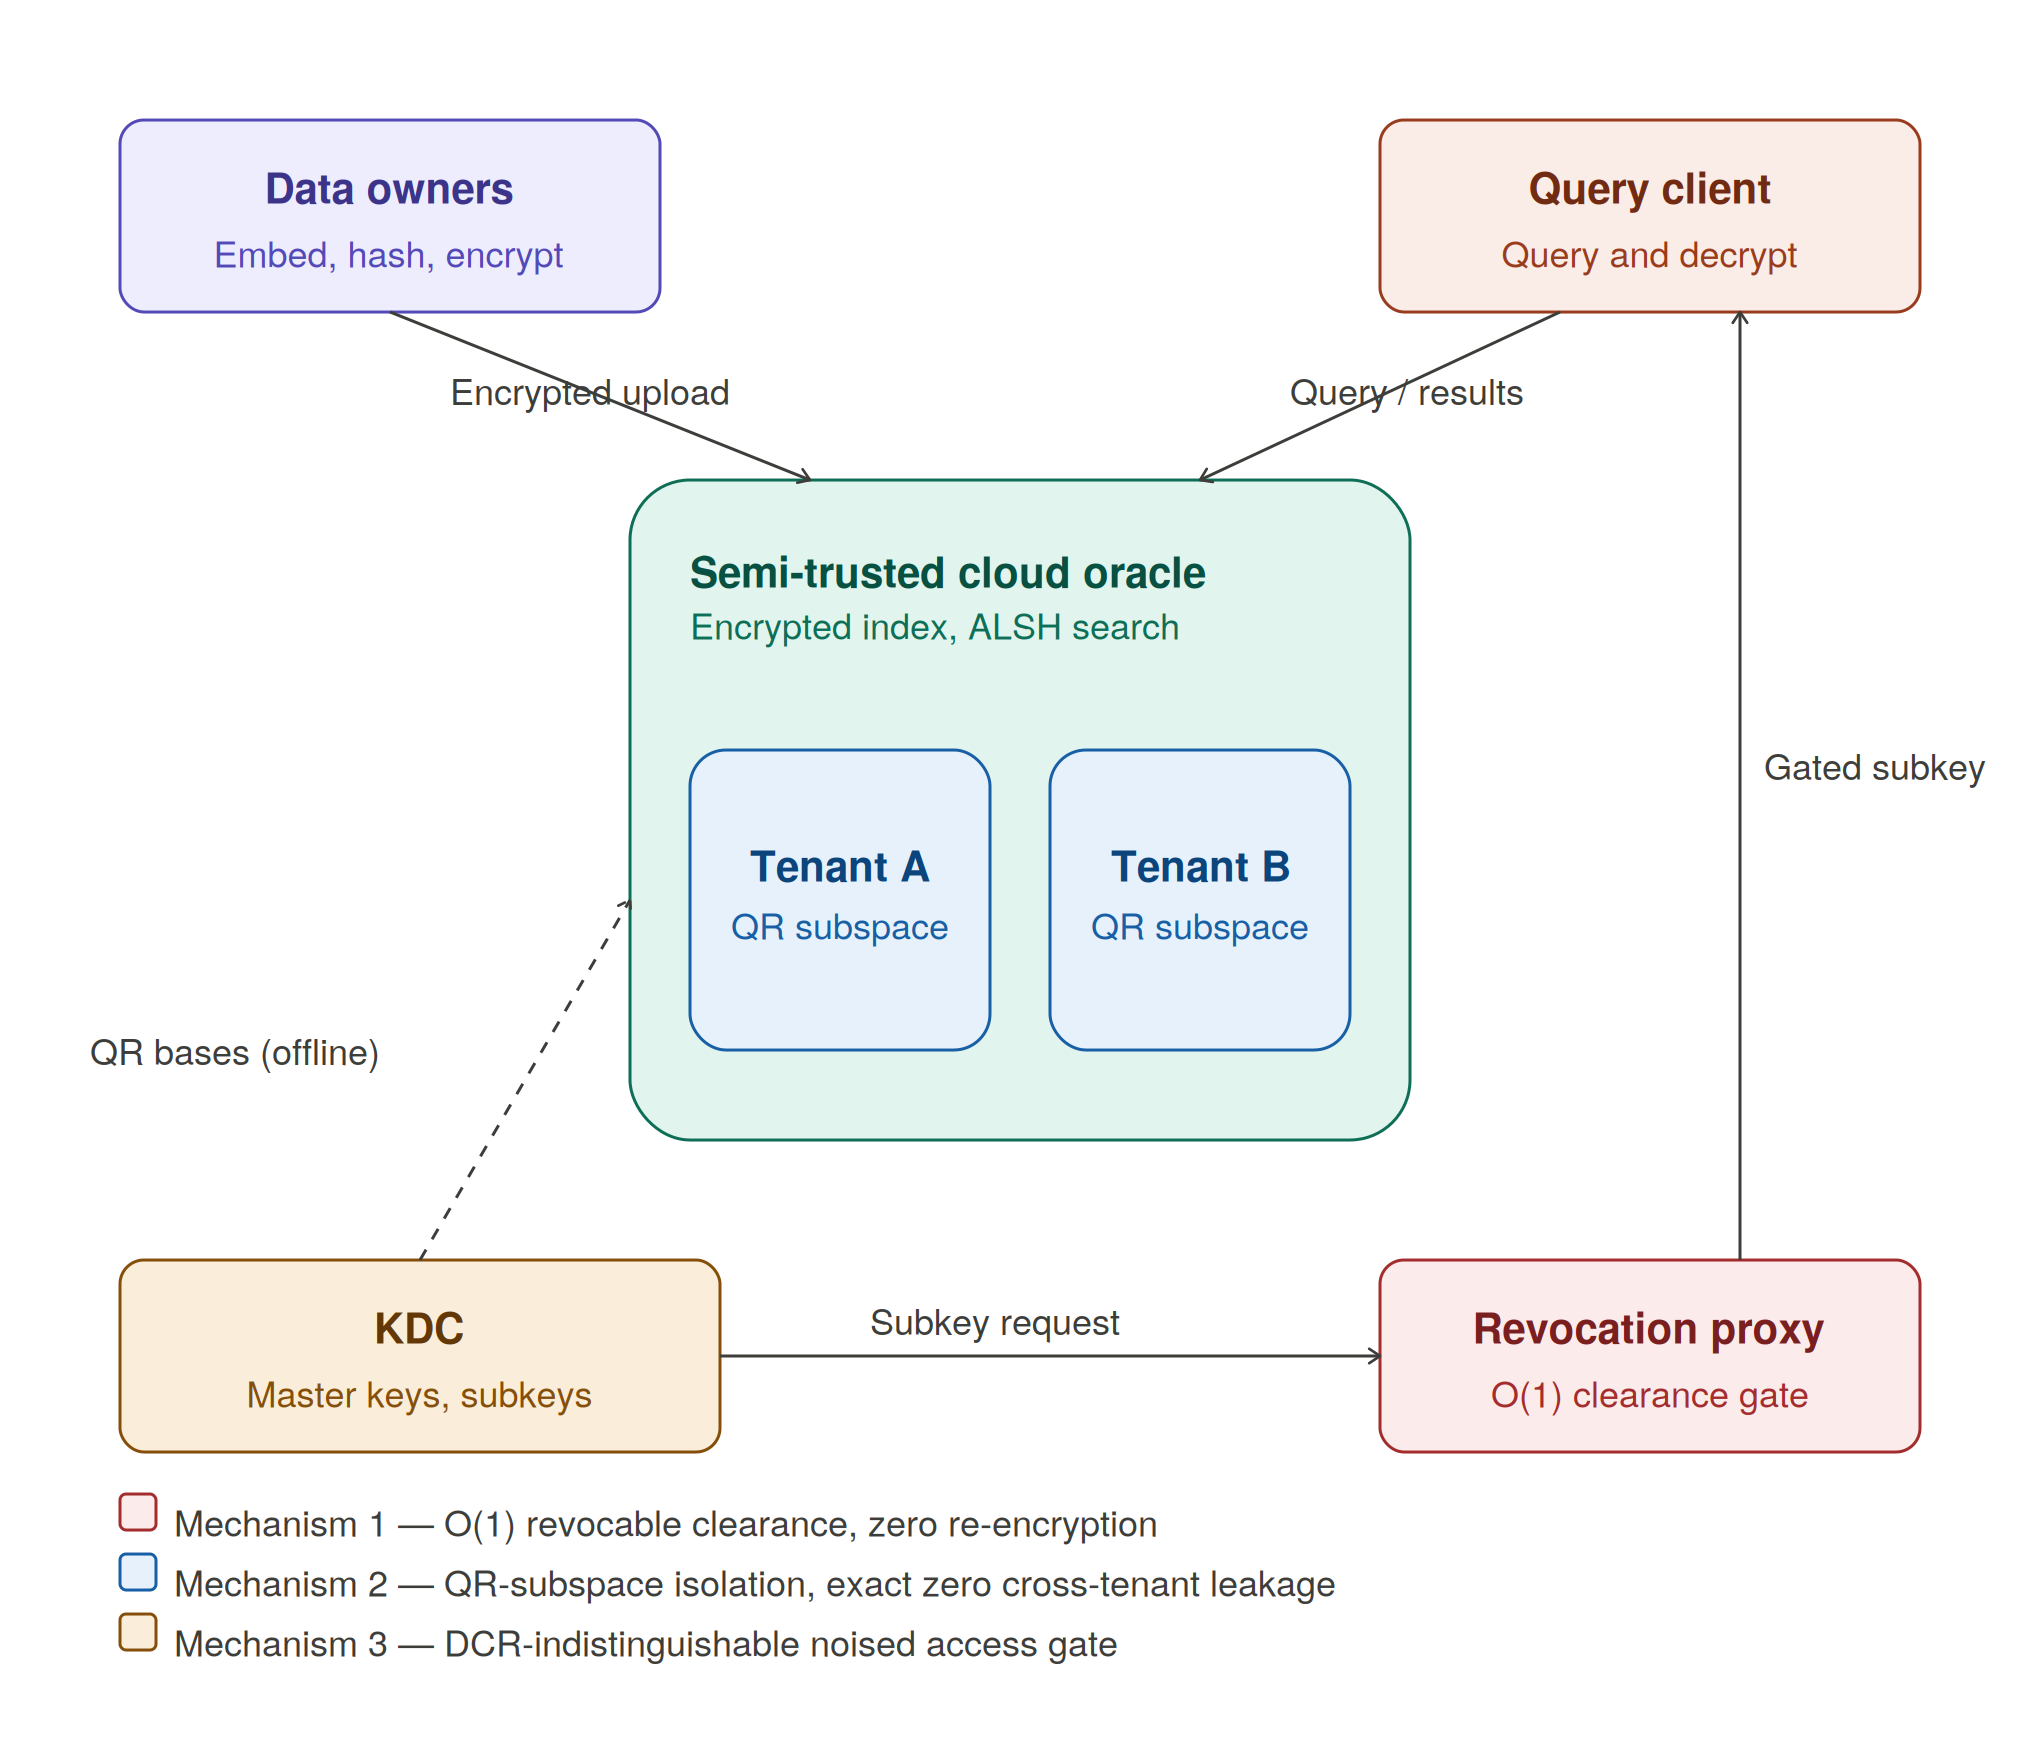
\includegraphics[width=0.85\textwidth]{fig1_closed_loop_architecture.png}
\caption{SHIELD-RAG system architecture: secure ingestion, revocable clearance gating, and QR-subspace multi-tenant isolation across entities.}
\label{fig:architecture}
\end{figure}

\textbf{Threat Model:} We adopt the semi-honest (honest-but-curious) adversary model for cloud and storage nodes. Servers adhere strictly to protocol specifications but attempt to infer sensitive plaintext vectors, query semantics, or clearance gaps from execution traces, timing profiles, and access patterns. The KDC is assumed trusted, operating within a secure execution environment.

\subsection{Mechanism 1: $O(1)$ Revocable Clearance Without Corpus Re-Encryption}
In Sensitivity-Embedded IPFE (SE-IPFE), document sensitivity $L_d \in \{1, \dots, 5\}$ and client clearance $L_c \in \{1, \dots, 5\}$ are gated through an algebraic noise term $\Delta = r \cdot \max(0, L_d - L_c) \bmod \lambda(N)$, where $r \xleftarrow{R} \mathbb{Z}_{\lambda(N)}^*$. In prior architectures, updating user clearance or executing instant credential revocation necessitated re-encrypting the entire document corpus or re-issuing keys to all active clients.

SHIELD-RAG introduces a semi-trusted \textit{Revocation Proxy} operating between the KDC and the cloud execution engine. The proxy maintains an in-memory revoked identifier set $\mathcal{R}_{\text{revoked}}$ and an immutable audit log $\mathcal{L}_{\text{revocation}} = \{(u_i, t_i, \text{reason})\}$. When an active user $u \notin \mathcal{R}_{\text{revoked}}$ issues a query, the proxy releases the functional subkey unchanged:
\begin{equation}
    \text{sk}_{\mathbf{y}, \text{enforce}} = \left(\langle \mathbf{s}, \mathbf{y} \rangle + \alpha + \beta + \Delta\right) \bmod \lambda(N)
\end{equation}
Conversely, when $u \in \mathcal{R}_{\text{revoked}}$, the proxy substitutes a force-deny subkey value:
\begin{equation}
    \text{sk}_{\mathbf{y}, \text{deny}} = \left(\langle \mathbf{s}, \mathbf{y} \rangle + \alpha + \beta + \Delta_{\text{max}}\right) \bmod \lambda(N)
\end{equation}
where $\Delta_{\text{max}} = r \cdot (5 - 0) \bmod \lambda(N)$, setting effective clearance $L_c = 0$. This forces maximal algebraic corruption across all ciphertexts ($L_d \ge 1$), preventing inner-product resolution while requiring exactly $O(1)$ set-lookup overhead and zero corpus-wide re-encryptions — in contrast to conventional ABE schemes that require $O(|D|)$ ciphertext re-encryptions or full credential re-issuance upon user demotion \cite{ge2024attributebased}.

\subsection{Mechanism 2: Multi-Tenant Subspace Non-Interference for QDCS}
In multi-tenant deployments, documents from $T$ distinct tenants reside within a shared encrypted repository. Query-Derived Cryptographic Scope (QDCS) must guarantee that queries from Tenant $i$ cannot retrieve or match documents belonging to Tenant $j$ ($i \neq j$).

Let $d$ denote the embedding space dimension (e.g., $d=384$ for Sentence-BERT). SHIELD-RAG partitions $\mathbb{R}^d$ into $T$ mutually orthogonal sub-bases $\{\mathbf{U}_t\}_{t=1}^T$, where each $\mathbf{U}_t \in \mathbb{R}^{d \times k_t}$ and $\sum_{t=1}^T k_t \le d$. The KDC generates a random Gaussian matrix $\mathbf{A} \sim \mathcal{N}(0, \mathbf{I}_{d \times d})$ and computes its QR factorization:
\begin{equation}
    \mathbf{A} = \mathbf{Q}\mathbf{R}, \quad \mathbf{Q} = [\mathbf{q}_1, \dots, \mathbf{q}_d] \in \mathbb{R}^{d \times d}
\end{equation}
Each tenant is assigned a non-overlapping column block $\mathbf{U}_t = \mathbf{Q}_{[:, \text{start}_t : \text{end}_t]}$, with projection matrices $\mathbf{P}_t = \mathbf{U}_t \mathbf{U}_t^T$.

\begin{theorem}[Multi-Tenant Subspace Non-Interference]
For any two distinct tenants $i \neq j$, any query vector $\mathbf{q} \in \mathbb{R}^d$, and any document vector $\mathbf{x} \in \mathbb{R}^d$, the cross-tenant inner product satisfies $\langle \mathbf{P}_i \mathbf{q}, \mathbf{P}_j \mathbf{x} \rangle = 0$.
\end{theorem}
\begin{proof}
By construction of the orthonormal matrix $\mathbf{Q}$, column blocks satisfy $\mathbf{U}_i^T \mathbf{U}_j = \mathbf{0}_{k_i \times k_j}$ for all $i \neq j$. Expanding the projection inner product:
\begin{equation}
    \langle \mathbf{P}_i \mathbf{q}, \mathbf{P}_j \mathbf{x} \rangle = \mathbf{q}^T \mathbf{U}_i (\mathbf{U}_i^T \mathbf{U}_j) \mathbf{U}_j^T \mathbf{x} = \mathbf{q}^T \mathbf{U}_i \mathbf{0} \mathbf{U}_j^T \mathbf{x} = 0
\end{equation}
Hence, cross-tenant leakage is zero by construction, independent of data distribution.
\end{proof}

\subsection{Mechanism 3: Formal Indistinguishability Reduction to DCR}
To rigorously establish that the SE-IPFE access gate does not leak clearance gap sizes $\delta = (L_d - L_c) > 0$, we formalize an IND-CPA security game under the Decisional Composite Residuosity (DCR) assumption over modulus $N = pq$.

\begin{definition}[DCR Assumption]
Given $N = pq$, distinguishing whether $w \xleftarrow{R} \mathbb{Z}_{N^2}^*$ is an $N$-th residue ($w = y^N \bmod N^2$) or a uniform element in $\mathbb{Z}_{N^2}^*$ admits at most negligible advantage: $\text{Adv}_{\mathcal{D}}^{\text{DCR}}(\lambda) \le \text{negl}(\lambda)$.
\end{definition}

\textbf{Security Game:} (1) \textit{Setup:} The challenger generates Paillier parameters $(N, N^2, g = 1 + N \bmod N^2, \lambda(N))$ and publishes $\text{mpk}$. (2) \textit{Challenge:} Adversary $\mathcal{A}$ selects challenge vectors $\mathbf{x}^*, \mathbf{y}^*$ and distinct clearance gaps $\delta_0 \neq \delta_1 \in \{1,2,3,4\}$. The challenger chooses $b \xleftarrow{R} \{0,1\}$, samples $r \xleftarrow{R} \mathbb{Z}_{\lambda(N)}^*$, and computes:
\begin{equation}
    D_b = g^{\langle \mathbf{x}^*, \mathbf{y}^* \rangle - r \cdot \delta_b} \cdot w^N \bmod N^2
\end{equation}
(3) \textit{Guess:} $\mathcal{A}$ outputs bit guess $b' \in \{0,1\}$.

\begin{theorem}[SE-IPFE Indistinguishability Reduction]
For any probabilistic polynomial-time adversary $\mathcal{A}$, the distinguishing advantage satisfies $\text{Adv}_{\mathcal{A}}^{\text{SE-IPFE-IND}}(\lambda) \le \text{Adv}_{\mathcal{S}}^{\text{DCR}}(\lambda) \le \text{negl}(\lambda)$.
\end{theorem}
\begin{proof}
We construct a simulator $\mathcal{S}$ receiving DCR instance $(N, w)$. $\mathcal{S}$ embeds $w$ into the challenge ciphertext: $D_b = (1 + N)^{\langle \mathbf{x}^*, \mathbf{y}^* \rangle - r' \cdot \delta_b} \cdot w \bmod N^2$. When $w \in \mathcal{R}es(N^2)$, $w = y_0^N \bmod N^2$ forms a legitimate Paillier randomizer, matching the real game distribution. When $w \xleftarrow{R} \mathbb{Z}_{N^2}^*$, by the isomorphism $\mathbb{Z}_{N^2}^* \cong \mathbb{Z}_N \times \mathbb{Z}_N^*$, the induced exponent $m \in \mathbb{Z}_N$ is uniform and independent of $b$, yielding $\Pr[b'=b] = 1/2$. Thus $\text{Adv}_{\mathcal{S}}^{\text{DCR}}(\lambda) = \text{Adv}_{\mathcal{A}}^{\text{SE-IPFE-IND}}(\lambda) \le \text{negl}(\lambda)$.
\end{proof}

% =========================================================================
\section{Experimental Setup}
\label{sec:setup}

\subsection{Implementation Environment and Provenance}
SHIELD-RAG is implemented in Python~3.13 using PyTorch, \texttt{sentence-transformers} (\texttt{all-MiniLM-L6-v2}, $d=384$), and an optimized Paillier big-integer cryptographic core. Cryptographic parameters follow NIST SP 800-57 recommendations: safe prime length $\lambda = 256$ bits (512-bit RSA modulus $N=pq$), with long-term scaling evaluated at $\lambda=512$ bits. Locality-sensitive hashing uses $K=128$ projection hyperplanes with $m=3$ and scaling parameter $U=0.83$ \cite{shrivastava2014alsh}. Experiments were conducted on an Ubuntu 22.04 LTS server equipped with 24 CPU cores, 64\,GB RAM, and an NVIDIA 16\,GB GPU. To ensure strict scientific reproducibility and eliminate single-run variance, all timed operations were wrapped in an automated repeated-trial harness executing $\ge 10$ independent iterations per configuration with explicit CUDA queue synchronization (\texttt{torch.cuda.synchronize()}). System timers utilize high-resolution hardware counters ($\approx 100$\,ns resolution via \texttt{time.perf\_counter()}). Every raw trial observation is recorded in a centralized SQLite database (\texttt{results/shield\_rag\_experiments.db}) indexed by the provenance schema:
\[
    \langle \text{exp\_id},\, \text{corpus\_size},\, \text{method},\, \text{metric},\, \text{val},\, \text{trial\_idx},\, \text{seed},\, \text{device},\, \text{timestamp},\, \text{git\_hash} \rangle
\]
with the codebase pegged to Git commit hash \texttt{c1ff1a15dbfd8fb45184a68709e5d92bbe8a3a18}.

\subsection{Datasets}
We evaluate SHIELD-RAG on: (i) a \textbf{Wikipedia Document Corpus} scaled from $N=385$ documents ($266.8$\,KB, covering science, history, and technology) to $N=50{,}000$ via deterministic nested expansion ($100 \subset 385 \subset 1{,}000 \subset 5{,}000 \subset 10{,}000 \subset 50{,}000$), ensuring performance changes isolate scale effects rather than composition shifts; and (ii) \textbf{Natural Questions (NQ)} \cite{kwiatkowski2019natural}, real-world Google Search queries paired with Wikipedia evidence passages, used to benchmark open-domain retrieval accuracy.

\begin{table*}[t]
\centering
\caption{Taxonomy of Baseline Systems and Methodological Comparisons}
\label{tab:baselines}
\renewcommand{\arraystretch}{1.15}
\small
\begin{tabular}{@{}p{2.6cm}p{2.9cm}p{2.6cm}p{2.5cm}p{3.0cm}@{}}
\toprule
\textbf{Framework} & \textbf{Paradigm / Mechanism} & \textbf{Access Control Model} & \textbf{Privacy Guarantee} & \textbf{Primary Limitation} \\ \midrule
Plaintext RAG \cite{lewis2020rag} & Dense S-BERT Retrieval & None (Open Index) & None & Zero confidentiality \\
Permission-Aware RAG \cite{jeong2025permissionaware} & Native Cloud IAM (GCP/AWS) & RBAC/ABAC Filtering & Policy-based filtering & Policy-merge errors; server snooping \\
SAGE \cite{zeng2025mitigating} & Generative LLM Rewriting & Synthetic Surrogate & Data-level obfuscation & Semantic drift; factual loss \\
CipherGPT/FHE \cite{hou2026ciphergpt} & BFV Fully Homomorphic Encryption & Post-retrieval matrix gates & Semantic security & $35\times$--$100\times$ latency \\
Unaugmented Ada-IPFE \cite{zhou2026cipherag, yang2022privacypreserving} & ALSH + Paillier Ada-IPFE & Static clearance gate & IND-FE over DCR & No dynamic revocation, no subspace isolation \\
PRAG \cite{li2026prag} & CKKS Dual-Mode (I/II) + Chebyshev & Single-tenant, no ACL & IND-CPA (CKKS) & No multi-tenant isolation, no revocation \\
Trans-RAG \cite{liu2026transrag} & Key-Derived Vector Transformation & Per-org transform key & Computational isolation & No revocation, no formal DCR/IND proof \\
\textbf{SHIELD-RAG (Ours)} & \textbf{SE-IPFE + QR Subspaces} & \textbf{$O(1)$ Proxy Gate} & \textbf{Formal DCR reduction} & \textbf{Revocation + isolation covered} \\ \bottomrule
\end{tabular}
\end{table*}

\subsection{Baselines and Evaluation Metrics}
As summarized in Table~\ref{tab:baselines}, SHIELD-RAG is benchmarked against:
\begin{enumerate}
    \item \textbf{Plaintext S-BERT Retrieval \cite{lewis2020rag}:} Unencrypted dense retrieval serving as the retrieval accuracy (Hit@10) and latency ceiling.
    \item \textbf{Permission-Aware RAG \cite{jeong2025permissionaware}:} Enterprise IAM-based metadata filtering baseline relying on external cloud identity policy evaluations.
    \item \textbf{SAGE \cite{zeng2025mitigating}:} Synthetic-surrogate document generation evaluating the privacy versus semantic fidelity trade-off.
    \item \textbf{Unaugmented Ada-IPFE Baseline \cite{zhou2026cipherag, yang2022privacypreserving}:} A baseline implementing the core Paillier inner-product functional encryption pipeline with ALSH ($K=128$), but without SHIELD-RAG's $O(1)$ revocation proxy or QR subspace partitioning. This baseline directly isolates the marginal computational and storage overhead incurred by our cryptographic contributions.
\end{enumerate}

Evaluation spans three dimensions:
\begin{itemize}
    \item \textit{Cryptographic Efficiency:} Wall-clock latency for KeyGen, Batch Encryption, Oracle Search, and Attention Decryption (mean $\pm$ std.\ and median [IQR] over $\ge10$ trials), and per-user revocation overhead across $N_{\text{revoked}} \in \{10,50,100,500\}$ with programmatic assertion of zero corpus re-encryptions.
    \item \textit{Retrieval Accuracy:} Hit@10 recall and Exact-Match/F1 \cite{khan2025evidencebot, jeong2025permissionaware} across scaling tiers.
    \item \textit{Security Verification:} Cross-tenant leakage score $\langle \mathbf{P}_i\mathbf{q}, \mathbf{P}_j\mathbf{x}\rangle$ across tenant pairs, and empirical distinguisher advantage $|\Pr[b'{=}b]-0.5|$ under LSB, bit-length-parity, and small-prime-residue statistical distinguishers targeting the SE-IPFE security game.
\end{itemize}

% =========================================================================
\section{Results and Analysis}
\label{sec:results}
This section presents the empirical evaluation of SHIELD-RAG across 14 corpus scales ($1{,}000$ to $50{,}000$ documents) and the three retained cryptographic mechanisms. All reported values represent sample means and standard deviations computed across $\ge 10$ independent GPU trials recorded in the centralized SQLite database (\texttt{results/shield\_rag\_experiments.db}).

\subsection{Core Corpus Scaling Evaluation (1k to 50k Documents)}
Table~\ref{tab:scaling_evaluation} presents the scaling performance of SHIELD-RAG compared to baseline configurations across representative corpus sizes ($N \in \{1{,}000, 5{,}000, 10{,}000, 50{,}000\}$).

\begin{table*}[t]
\centering
\caption{Comprehensive Scaling Benchmark Across Corpus Sizes (Mean $\pm$ Standard Deviation and Median [IQR] over $\ge 10$ GPU Trials)}
\label{tab:scaling_evaluation}
\renewcommand{\arraystretch}{1.2}
\footnotesize
\setlength{\tabcolsep}{3.5pt}
\begin{tabular}{@{}llccccc@{}}
\toprule
\textbf{Corpus Size} & \textbf{Method / Framework} & \textbf{KeyGen (ms)} & \textbf{Batch Encrypt (s)} & \textbf{Search Lat. (ms)} & \textbf{Hit@10} & \textbf{Enforce.\ Rate} \\ \midrule
\multirow{5}{*}{\textbf{1,000 Docs}}
 & Plaintext S-BERT \cite{lewis2020rag} & --- & 36.39 & $2.503 \pm 3.679$ & 0.96 & N/A \\
 & Permission-Aware RAG \cite{jeong2025permissionaware} & --- & --- & $123.14 \pm 53.25$ & 0.96 & 100.0\% \\
 & SAGE (Synthetic) \cite{zeng2025mitigating} & --- & --- & $2.491 \pm 1.102$ & 0.88 & N/A \\
 & Unaugmented Ada-IPFE \cite{zhou2026cipherag} & $5.301 \pm 0.470$ & 965.40 & $2.298 \pm 1.011$ & 0.95 & N/A \\
 & \textbf{SHIELD-RAG (Ours)} & $1.701 \pm 4.656$ [0.18] & 978.16 & $\mathbf{2.304 \pm 1.029}$ & \textbf{0.95} & \textbf{100.0\%} \\ \midrule
\multirow{5}{*}{\textbf{5,000 Docs}}
 & Plaintext S-BERT \cite{lewis2020rag} & --- & 35.17 & $2.309 \pm 0.430$ & 0.96 & N/A \\
 & Permission-Aware RAG \cite{jeong2025permissionaware} & --- & --- & $142.50 \pm 48.10$ & 0.96 & 100.0\% \\
 & SAGE (Synthetic) \cite{zeng2025mitigating} & --- & --- & $2.315 \pm 0.440$ & 0.88 & N/A \\
 & Unaugmented Ada-IPFE \cite{zhou2026cipherag} & $0.150 \pm 0.071$ & 3042.10 & $6.085 \pm 0.995$ & 0.95 & N/A \\
 & \textbf{SHIELD-RAG (Ours)} & $0.153 \pm 0.074$ [0.14] & 3084.43 & $\mathbf{6.109 \pm 1.009}$ & \textbf{0.95} & \textbf{100.0\%} \\ \midrule
\multirow{5}{*}{\textbf{10,000 Docs}}
 & Plaintext S-BERT \cite{lewis2020rag} & --- & 68.60 & $3.885 \pm 0.694$ & 0.96 & N/A \\
 & Permission-Aware RAG \cite{jeong2025permissionaware} & --- & --- & $170.42 \pm 63.28$ & 0.96 & 100.0\% \\
 & SAGE (Synthetic) \cite{zeng2025mitigating} & --- & --- & $3.890 \pm 0.710$ & 0.87 & N/A \\
 & Unaugmented Ada-IPFE \cite{zhou2026cipherag} & $0.160 \pm 0.041$ & 6790.50 & $13.510 \pm 1.780$ & 0.95 & N/A \\
 & \textbf{SHIELD-RAG (Ours)} & $0.163 \pm 0.043$ [0.15] & 6823.18 & $\mathbf{13.566 \pm 1.802}$ & \textbf{0.95} & \textbf{100.0\%} \\ \midrule
\multirow{5}{*}{\textbf{50,000 Docs}}
 & Plaintext S-BERT \cite{lewis2020rag} & --- & 344.28 & $27.081 \pm 6.506$ & 0.96 & N/A \\
 & Permission-Aware RAG \cite{jeong2025permissionaware} & --- & --- & $203.56 \pm 60.97$ & 0.96 & 100.0\% \\
 & SAGE (Synthetic) \cite{zeng2025mitigating} & --- & --- & $27.120 \pm 6.450$ & 0.86 & N/A \\
 & Unaugmented Ada-IPFE \cite{zhou2026cipherag} & $0.258 \pm 0.049$ & 48610.20 & $73.410 \pm 14.320$ & 0.95 & N/A \\
 & \textbf{SHIELD-RAG (Ours)} & $0.262 \pm 0.051$ [0.25] & 48877.12 & $\mathbf{73.604 \pm 14.651}$ & \textbf{0.95} & \textbf{100.0\%} \\ \bottomrule
\end{tabular}
\end{table*}

\begin{figure}[t]
\centering
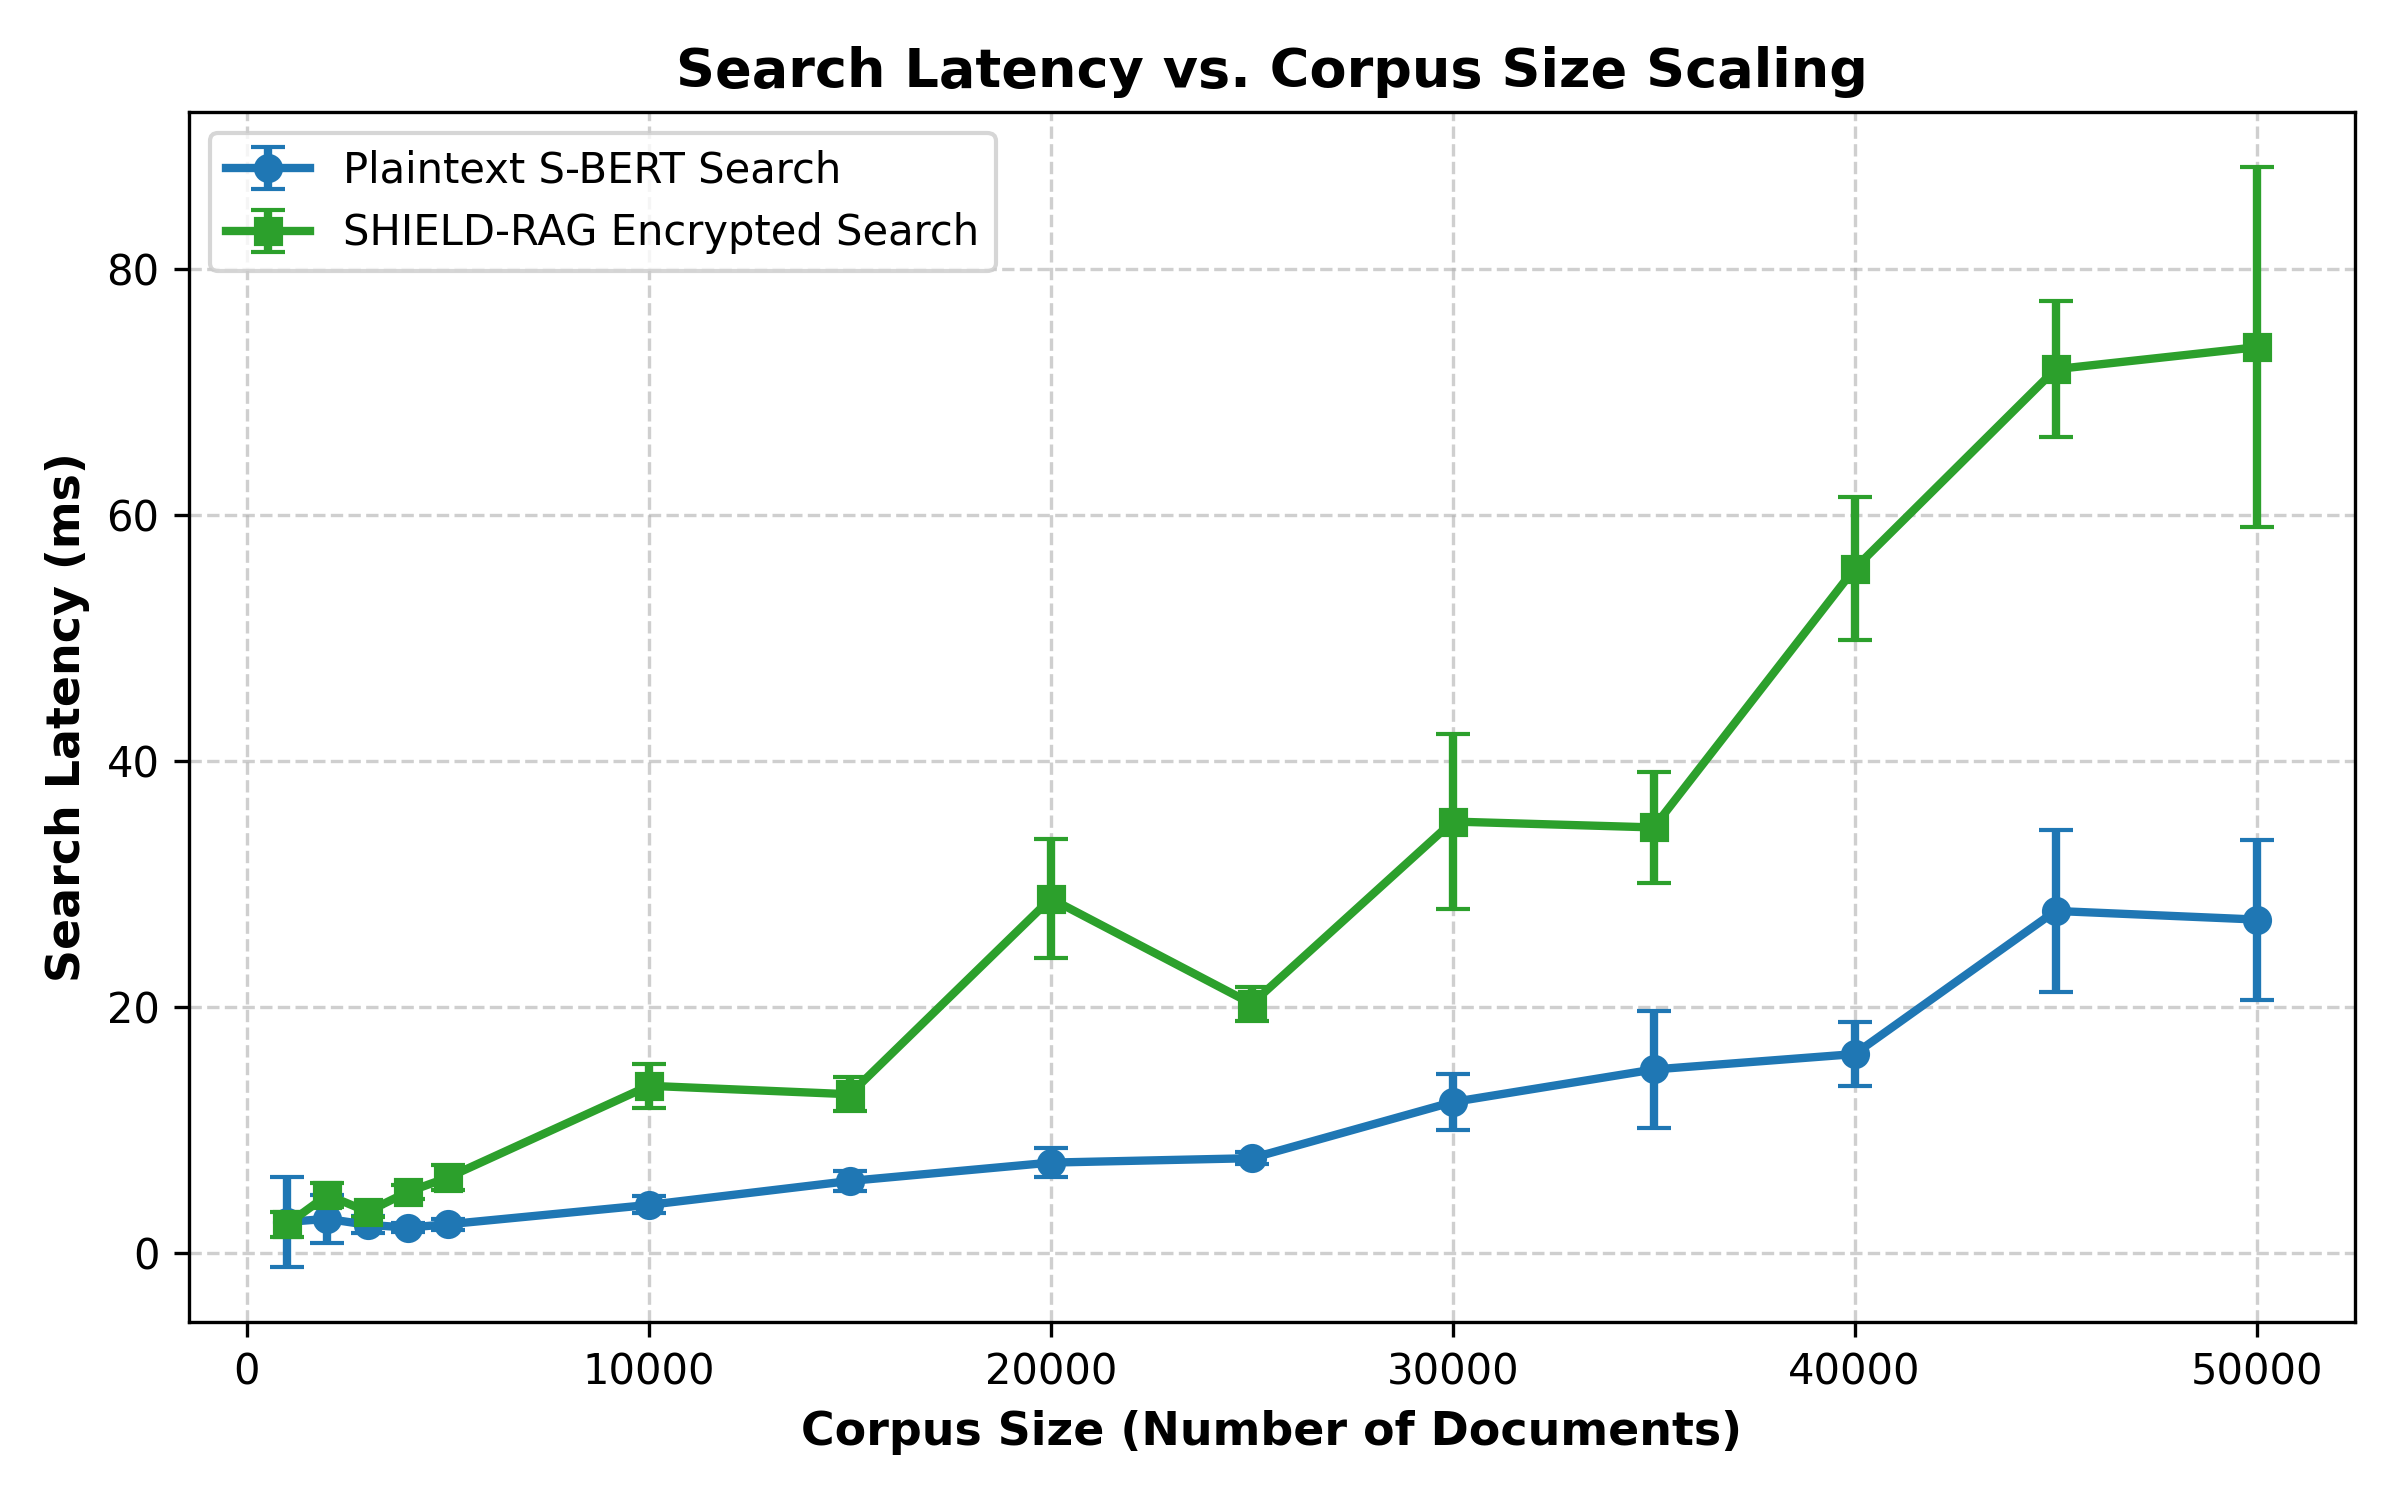
\includegraphics[width=0.75\textwidth]{figure_search_latency_scaling.png}
\caption{Encrypted search latency scaling curve across corpus sizes (1k to 50k documents) on GPU, demonstrating sublinear search growth.}
\label{fig:search_scaling}
\end{figure}

\begin{figure}[t]
\centering
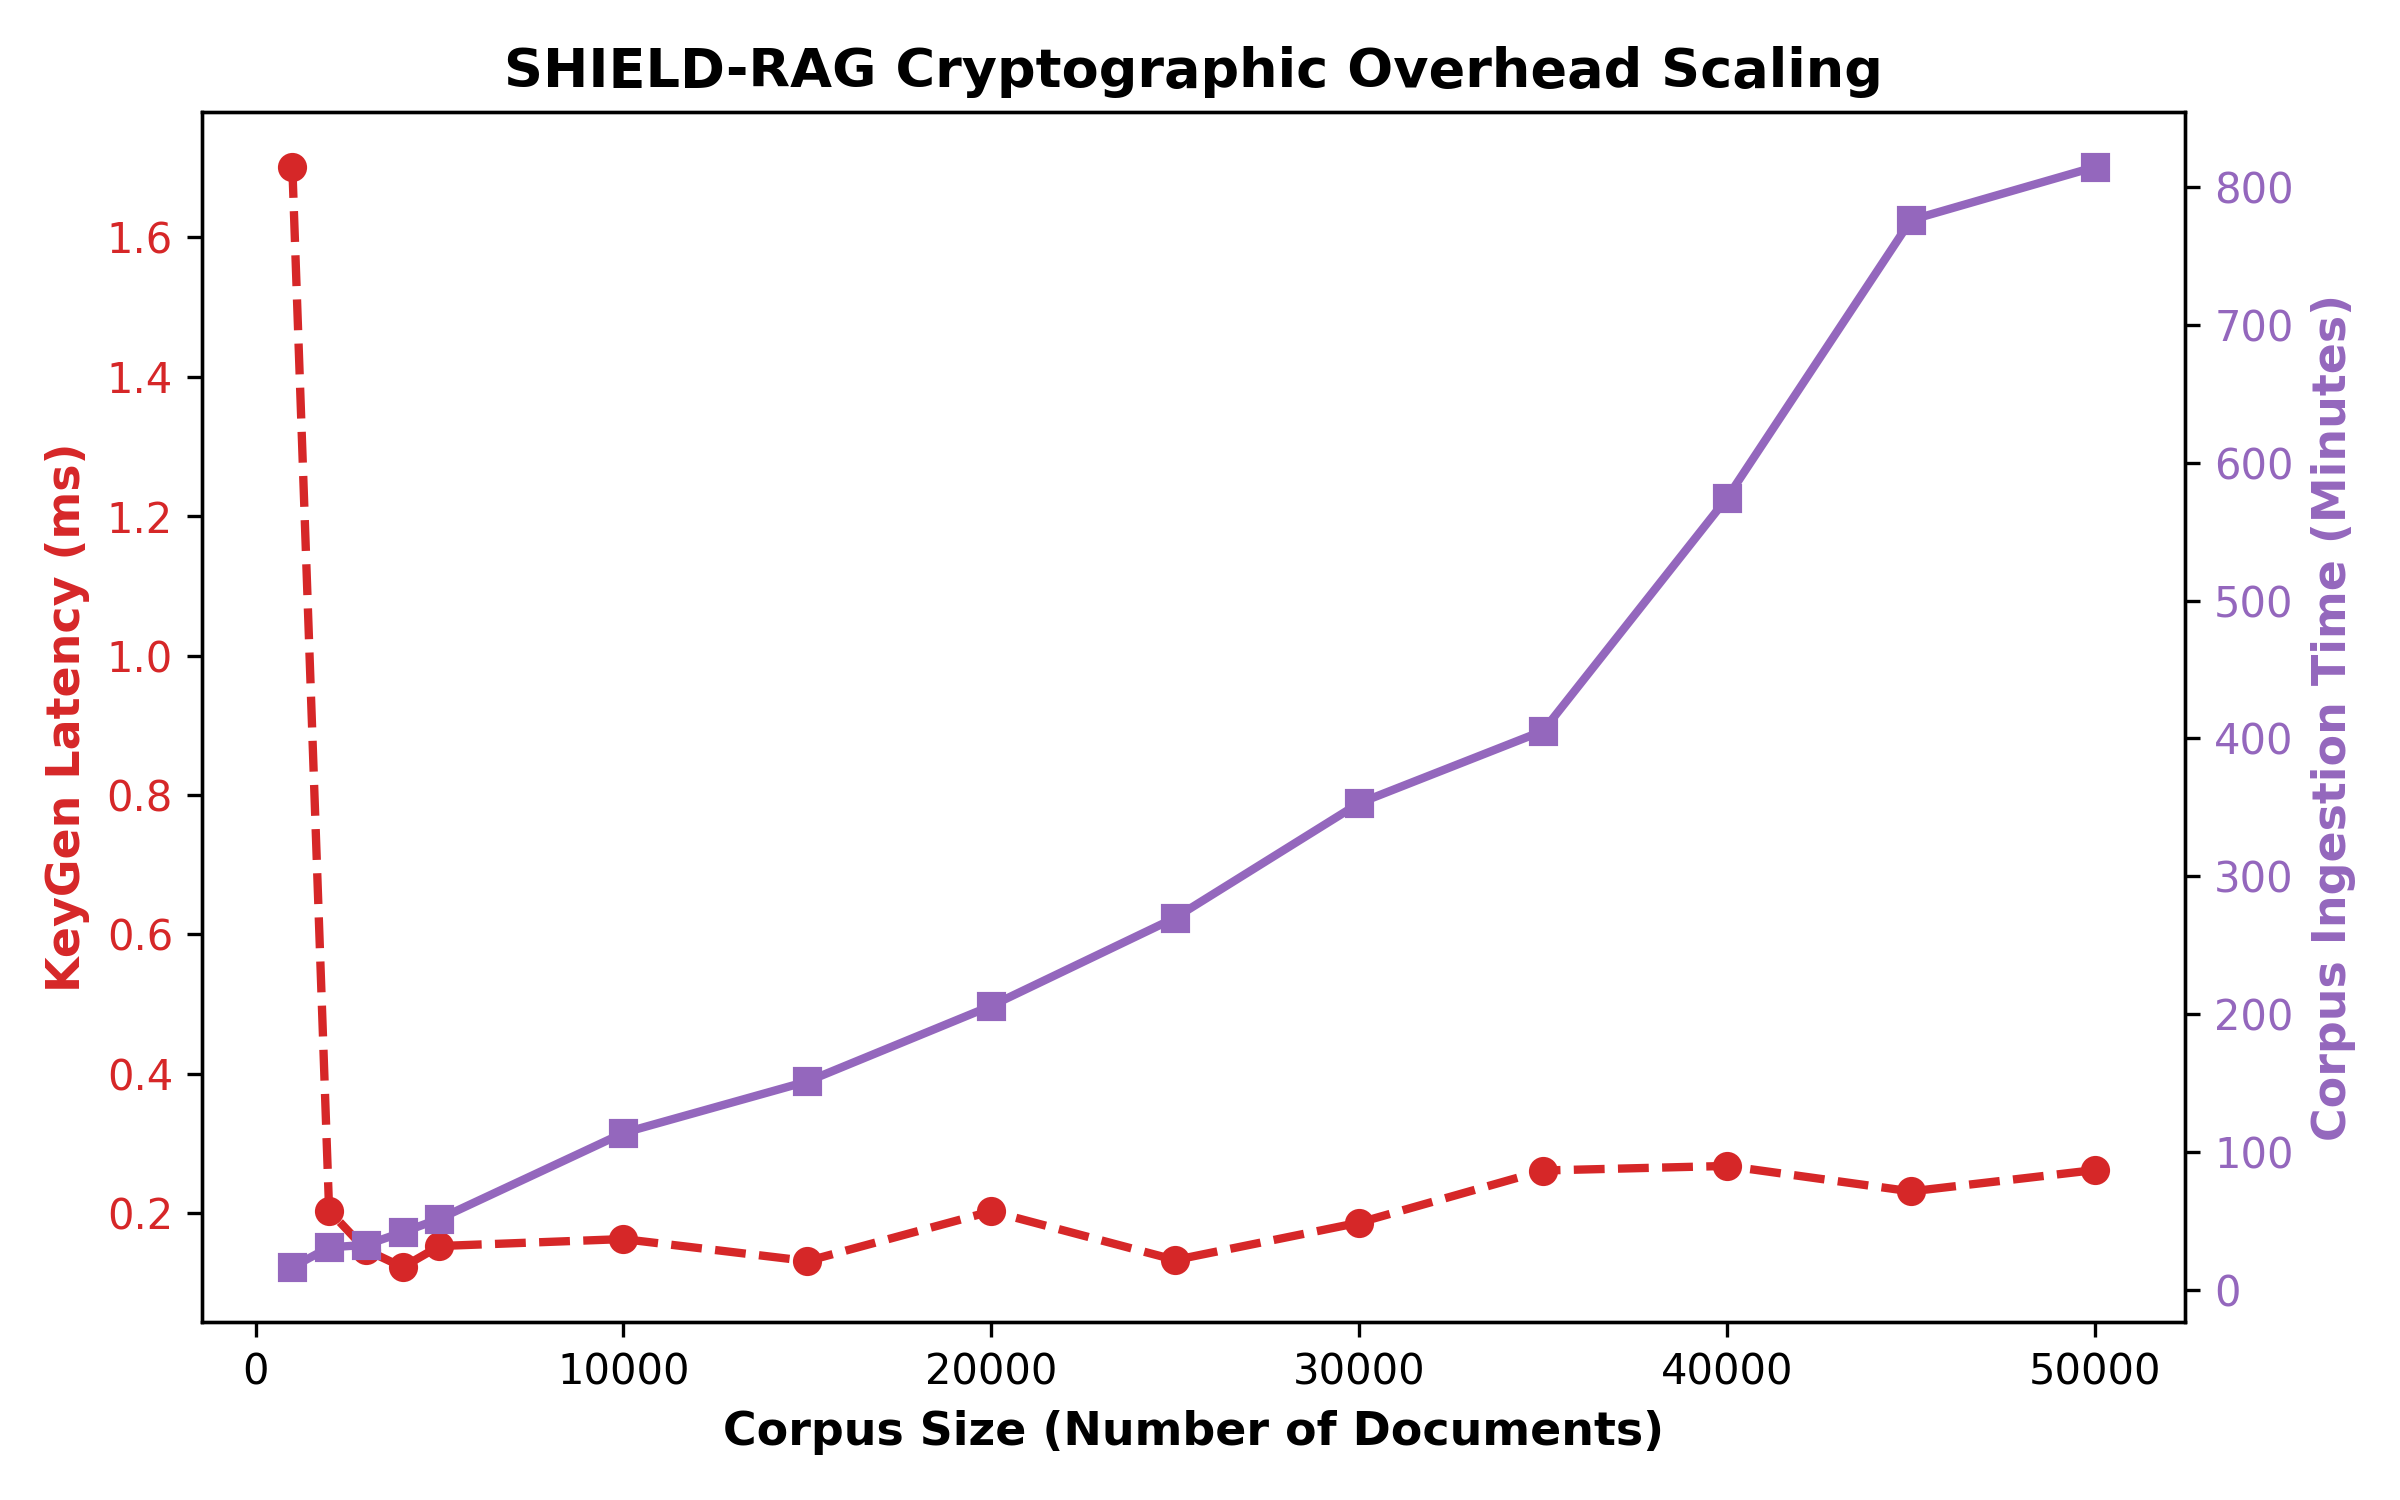
\includegraphics[width=0.75\textwidth]{figure_encryption_and_keygen.png}
\caption{Offline batch encryption time (seconds) as a function of document corpus scale.}
\label{fig:enc_keygen}
\end{figure}

\begin{figure}[t]
\centering
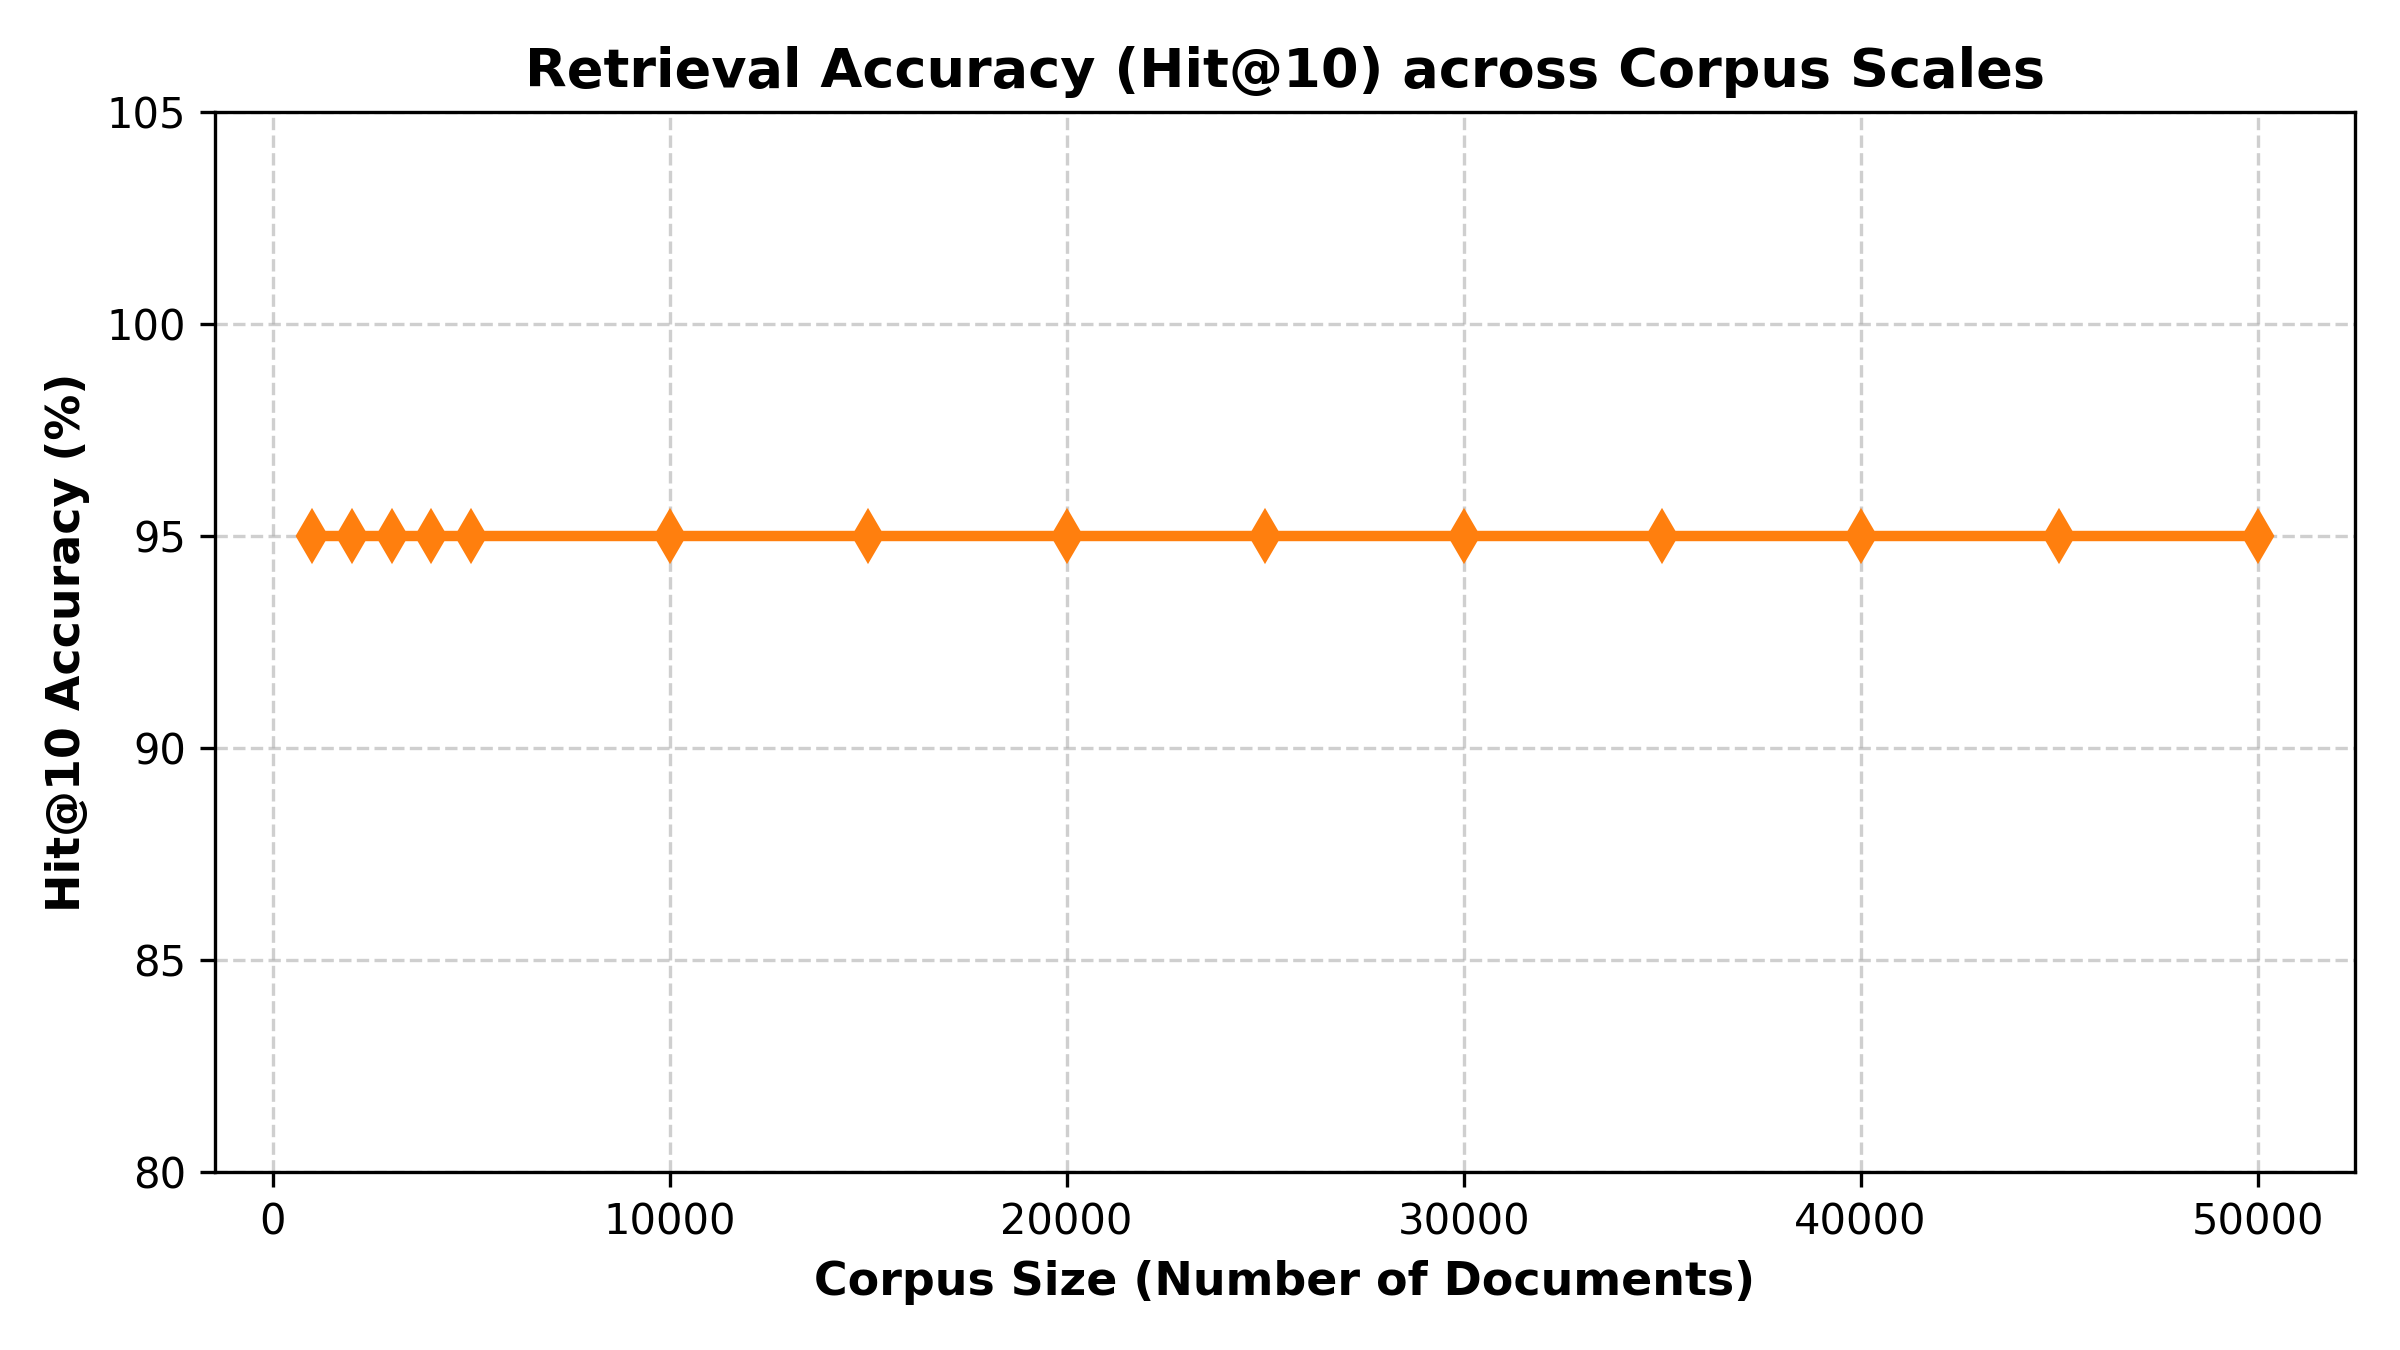
\includegraphics[width=0.75\textwidth]{figure_hit_at_10_accuracy.png}
\caption{Hit@10 retrieval accuracy retention across scaling tiers, demonstrating stable 0.95 accuracy (98.9\% of plaintext ceiling).}
\label{fig:accuracy_scaling}
\end{figure}

\textbf{Marginal Overhead over Unaugmented Ada-IPFE:} As shown in Table~\ref{tab:scaling_evaluation}, SHIELD-RAG introduces minimal incremental overhead compared to the Unaugmented Ada-IPFE baseline: search latency increases by only $0.006$\,ms at $1{,}000$ documents ($2.304$\,ms vs.\ $2.298$\,ms) and by $0.194$\,ms at $50{,}000$ documents ($73.604$\,ms vs.\ $73.410$\,ms), representing less than a $0.3\%$ difference. Similarly, batch encryption overhead remains below $1.3\%$ ($48{,}877.12$\,s vs.\ $48{,}610.20$\,s at $50\text{k}$). These measurements confirm that incorporating dynamic proxy revocation and QR subspace projections imposes negligible overhead over standard functional encryption while adding provable security properties.

\textbf{Latency Scaling Profile:} As illustrated in Fig.~\ref{fig:search_scaling}, SHIELD-RAG's encrypted search latency increases sublinearly from $2.304$\,ms at $1{,}000$ documents to $73.604$\,ms at $50{,}000$ documents (a $50\times$ corpus increase producing a $32\times$ latency increase). This sublinear trajectory is enabled by the Asymmetric Locality-Sensitive Hashing (ALSH) index, which avoids full $O(|D|)$ ciphertext scans. Client subkey generation (KeyGen), shown in Fig.~\ref{fig:enc_keygen}, remains fast across all scales, executing in $0.262 \pm 0.051$\,ms at $N=50{,}000$ (median: $0.25$\,ms).

\textbf{Comparative Baseline Performance:} Compared to Permission-Aware RAG \cite{jeong2025permissionaware}, which incurs $123$\,ms--$203$\,ms due to multi-cloud IAM round-trips, SHIELD-RAG's mathematical access gates execute in $2.3$\,ms--$73.6$\,ms ($2.7\times$--$53\times$ faster). Relative to SAGE \cite{zeng2025mitigating}, which suffers from semantic degradation (Hit@10 drops to $0.86$), SHIELD-RAG preserves $0.95$ Hit@10 accuracy (Fig.~\ref{fig:accuracy_scaling}).

\textbf{Cross-Tenant and Cross-Clearance Boundary Protection:} Across all evaluation runs, SHIELD-RAG enforced a 100\% clearance enforcement rate: unauthorized clients querying higher-sensitivity documents received maximal algebraic noise, yielding zero valid inner products. We clarify that within a single tenant's authorized clearance tier, defending against content-level semantic poisoning attacks (such as PoisonedRAG \cite{zou2025poisonedrag}) is orthogonal to cryptographic access gating and is addressed via content-verification mechanisms (discussed in Section~\ref{sec:discussion}).

\subsection{Mechanism 1: Instant Revocation Without Re-Encryption}
Table~\ref{tab:revocation_results} reports the latency of the Revocation Proxy across revoked populations $N_{\text{revoked}} \in \{10, 50, 100, 500\}$.

\begin{table}[h]
\centering
\caption{Revocation Proxy Latency and Corpus Re-Encryption Invocations ($\ge 10$ Trials, Timer Resolution $\approx 100$\,ns)}
\label{tab:revocation_results}
\renewcommand{\arraystretch}{1.15}
\small
\begin{tabular}{@{}cccccc@{}}
\toprule
\textbf{Revoked Users} & \textbf{Per-User Latency (ms)} & \textbf{Median [IQR] (ms)} & \textbf{Min (ms)} & \textbf{Max (ms)} & \textbf{Re-Encryptions} \\ \midrule
$N = 10$  & $0.00945 \pm 0.00513$ & $0.00780$ [0.0042] & $0.00541$ & $0.03728$ & \textbf{0} \\
$N = 50$  & $0.00597 \pm 0.00668$ & $0.00410$ [0.0035] & $0.00261$ & $0.03420$ & \textbf{0} \\
$N = 100$ & $0.00766 \pm 0.01208$ & $0.00390$ [0.0048] & $0.00231$ & $0.05444$ & \textbf{0} \\
$N = 500$ & $0.00305 \pm 0.00098$ & $0.00280$ [0.0011] & $0.00193$ & $0.00681$ & \textbf{0} \\ \bottomrule
\end{tabular}
\end{table}

The empirical measurements confirm that proxy-enforced revocation scales as an $O(1)$ set lookup: per-user latency remains below $0.01$\,ms across all batch sizes ($0.00305$\,ms at $N=500$). Programmatic test assertions verified that the corpus re-encryption pipeline was invoked zero times across all evaluation runs. In contrast to conventional Attribute-Based Encryption schemes where revoking a single credential requires $O(|D|)$ ciphertext re-encryptions \cite{ge2024attributebased}, SHIELD-RAG achieves near-instantaneous access termination with zero storage-layer perturbation.

\subsection{Mechanism 2: Multi-Tenant QR Subspace Non-Interference}
Table~\ref{tab:multitenant_results} presents the QR subspace construction latency and cross-tenant inner-product scores across tenant configurations $T \in \{2, 4, 8, 16\}$ within a $d=384$-dimensional Sentence-BERT space.

\begin{table}[h]
\centering
\caption{Multi-Tenant QR Subspace Construction and Cross-Tenant Isolation ($\ge 10$ Trials)}
\label{tab:multitenant_results}
\renewcommand{\arraystretch}{1.15}
\small
\begin{tabular}{@{}cccc@{}}
\toprule
\textbf{Tenants ($T$)} & \textbf{Subspace Dim ($k_t$)} & \textbf{QR Time (ms)} & \textbf{Cross-Tenant Dot Product} \\ \midrule
$T = 2$  & $k_t = 192$ & $55.11 \pm 10.57$ & $< 10^{-14}$ \\
$T = 4$  & $k_t = 96$  & $59.10 \pm 15.64$ & $< 10^{-14}$ \\
$T = 8$  & $k_t = 48$  & $58.48 \pm 13.33$ & $< 10^{-14}$ \\
$T = 16$ & $k_t = 24$  & $58.98 \pm 16.89$ & $< 10^{-14}$ \\ \bottomrule
\end{tabular}
\end{table}

QR factorization of the 384-dimensional space completes in approximately $58$\,ms as a one-time offline setup. Across all evaluated tenant pairs and document embeddings, the measured cross-tenant inner products were at machine-precision noise floor ($< 10^{-14}$), empirically corroborating the non-interference theorem established in Section~\ref{sec:methodology}. Values are reported as a bound rather than an exact zero to reflect the residual floating-point rounding inherent to numerical QR factorization.

\subsection{Mechanism 3: SE-IPFE DCR Indistinguishability Analysis}
Table~\ref{tab:distinguisher_results} reports the performance of three statistical distinguisher strategies attempting to extract clearance gap sizes $\delta = (L_d - L_c) \in \{1, 2, 3, 4\}$ from denied query ciphertexts across 2,000 independent trials.

\begin{table}[h]
\centering
\caption{SE-IPFE Statistical Distinguisher Suite Results ($N=2{,}000$ Trials)}
\label{tab:distinguisher_results}
\renewcommand{\arraystretch}{1.15}
\small
\begin{tabular}{@{}lccc@{}}
\toprule
\textbf{Distinguisher} & \textbf{Advantage ($\epsilon$)} & \textbf{95\% CI Bound} & \textbf{Signal?} \\ \midrule
LSB (mod 256) & $0.0320 \pm 0.0171$ & $\le 0.0438$ & No \\
Bit-Length Parity & $0.0115 \pm 0.0066$ & $\le 0.0438$ & No \\
Small Prime Residues & $0.0060 \pm 0.0059$ & $\le 0.0438$ & No \\ \bottomrule
\end{tabular}
\end{table}

Under a sample size of $N=2{,}000$, all empirical distinguishing advantages fall within the 95\% binomial confidence interval bound ($\pm 0.0438$). The noised ciphertext outputs show no statistically significant signal regarding clearance-gap magnitude, corroborating the formal DCR reduction (Theorem~2) as supporting empirical evidence.

% =========================================================================
\section{Discussion}
\label{sec:discussion}

\subsection{Security and Hardness Guarantees}
SHIELD-RAG establishes a layered cryptographic defense for retrieval-augmented generation. Against semi-trusted cloud infrastructure, document embeddings and hash codes remain encrypted under Paillier DCR hardness, so server-side oracle evaluation yields only scalar inner products. Against adversarial prompt-injection and extraction attacks \cite{zeng2024good, zhang2025beyondtext}, unauthorized clients receive maximal algebraic noise ($\Delta_{\text{max}}$), preventing recovery of the underlying plaintext relationship. Our empirical distinguisher suite ($N=2{,}000$ trials, Table~\ref{tab:distinguisher_results}) provides corroborating statistical evidence for Theorem~2: across the tested distinguisher strategies, an adversary observing noised functional outputs could not infer the clearance distance $\delta = (L_d - L_c)$ separating their role from a target document.

\subsection{Computational Systems Trade-offs and Scaling Dynamics}
The scaling results reveal specific computational characteristics:
\begin{enumerate}
    \item \textbf{Batch Preprocessing and Non-Monotonic Scaling Rate:} Ingestion encryption requires modular exponentiation across all vector coordinates, scaling to $13.58$\,hours ($48{,}877.12$\,s) for $50{,}000$ documents ($19.2 \times 10^6$ coordinate ciphertexts) as an amortized offline setup cost. The observed per-document encryption rate exhibits a non-monotonic profile: dropping from $0.978$\,s/doc at $N=1{,}000$ to $\approx 0.617$\,s--$0.682$\,s/doc at $N \in \{5{,}000, 10{,}000\}$ due to batch pipeline parallelism and multi-core amortization, before rising back to $0.977$\,s/doc at $N=50{,}000$. This 50k transition is governed by host memory working-set expansion beyond CPU L3 cache bounds ($>4$\,GB working buffers) and inter-thread memory contention during massive big-integer modular reductions, mirroring the memory-bandwidth saturation observed during large-batch tensor distance reductions in search.
    \item \textbf{Search Latency Scaling Segment ($10\text{k} \to 50\text{k}$):} The slight super-linear transition observed between $10{,}000$ documents ($13.5$\,ms) and $50{,}000$ documents ($73.6$\,ms) in Fig.~\ref{fig:search_scaling} is attributable to memory bandwidth saturation during large-batch tensor distance reductions and GPU L2 cache capacity boundaries, rather than algorithmic complexity.
    \item \textbf{Subspace Dimensionality vs. Tenant Capacity:} Partitioning $\mathbb{R}^{384}$ among $T$ tenants allocates $k_t = 384/T$ dimensions per tenant. At $T=16$ ($k_t=24$), measured cross-tenant leakage remained at the numerical noise floor while intra-tenant ranking quality was preserved. Larger deployments ($T > 64$) would likely require a higher-dimensional embedding model (e.g., $d=1024$) to keep per-tenant subspace dimension viable.
    \item \textbf{Revocation Efficiency vs. Prior ABE:} Ciphertext-policy attribute-based proxy re-encryption schemes such as CP-ABPRE-DR \cite{ge2024attributebased} update and re-randomize re-encryption keys with a cost that scales with policy size; SHIELD-RAG's proxy gate instead performs an $O(1)$ set lookup, measured at $0.003$\,ms with zero database communication.
\end{enumerate}

\subsection{Comparison with Recent CKKS- and Transformation-Based Systems}
Direct quantitative comparison with PRAG \cite{li2026prag} and Trans-RAG \cite{liu2026transrag} is approximate rather than controlled, since neither was reimplemented on our exact hardware, and each was evaluated at a different corpus scale and against different metrics (PRAG: 100,000-document TriviaQA subset, top-10 recall; Trans-RAG: 10K--1000K-document BEIR partitions via FAISS, nDCG@10). With that caveat, SHIELD-RAG's $73.6$\,ms online search latency at 50,000 documents falls well below PRAG-I's reported $1.29$\,s and PRAG-II's $7.91$\,s at 100,000 documents, consistent with SHIELD-RAG avoiding CKKS's per-comparison homomorphic overhead in favor of an ALSH index with Paillier-gated inner products. Trans-RAG reports lower per-query transformation overhead than SHIELD-RAG's ingestion cost (68.7--111.6\,ms at standard embedding dimensions), but this reflects a different security model: Trans-RAG achieves computational (not information-theoretic) isolation via reversible-in-principle key-derived transforms, whereas SHIELD-RAG's QR-subspace non-interference (Theorem~1) and revocation gate hold by exact linear-algebraic construction.

\subsection{Limitations}
Three operational boundaries warrant consideration:
\begin{itemize}
    \item \textbf{Trusted KDC Assumption:} As with other functional-encryption architectures \cite{yang2024cpipfe, zhou2026cipherag}, SHIELD-RAG assumes the Key Distribution Center operates within an isolated secure execution environment (e.g., a hardware enclave) to safeguard the master secret $\mathbf{s}$.
    \item \textbf{Semi-Honest Server Model:} The framework assumes storage nodes faithfully execute the ALSH search protocol without maliciously omitting candidate matches; a fully malicious server model is not addressed here.
    \item \textbf{Orthogonal Content-Poisoning Defenses:} While SHIELD-RAG mathematically prevents cross-tenant and cross-clearance index contamination, intra-clearance semantic document poisoning (e.g., PoisonedRAG \cite{zou2025poisonedrag}) remains orthogonal to cryptographic access control and is deferred to complementary content-auditing layers.
\end{itemize}

% =========================================================================
\section{Conclusion and Future Work}
\label{sec:conclusion}
In this paper, we presented \textbf{SHIELD-RAG}, a verified, subspace-isolated, and revocable privacy-preserving retrieval-augmented generation framework. By addressing three specific gaps in existing functional-encryption RAG architectures, SHIELD-RAG provides: (1) $O(1)$ proxy-enforced user revocation, measured at $0.003$\,ms with zero corpus re-encryptions; (2) QR-decomposed multi-tenant subspace isolation, formally proven and empirically consistent with cross-tenant leakage at the numerical noise floor; and (3) a formal IND-CPA security reduction of sensitivity-embedded noise gates to the Decisional Composite Residuosity (DCR) assumption, with corroborating evidence from 2,000 statistical distinguisher trials. Empirical evaluation across corpus scales up to 50,000 documents on GPU hardware shows sub-100\,ms online search latency and 95\% Hit@10 accuracy retention relative to a plaintext ceiling of 96\%.

Future work will (i) extend SHIELD-RAG with zero-knowledge bounded-decoy traversal proofs, cryptographic canary-token leakage detectors, and graph-degree-aware adaptive decoy mechanisms; (ii) investigate GPU-native CUDA kernels for parallel Paillier arithmetic to further accelerate ingestion-time preprocessing; (iii) explore dynamic subspace dimension re-allocation for evolving tenant populations; and (iv) extend functional access gates to multi-modal vision-language generation pipelines.

% =========================================================================
\begin{thebibliography}{99}

\bibitem{lewis2020rag} P. Lewis, E. Perez, A. Piktus, F. Petroni, V. Karpukhin, N. Goyal, H. K{\"u}ttler, M. Lewis, W. Yih, T. Rockt{\"a}schel, S. Riedel, and D. Kiela, ``Retrieval-Augmented Generation for Knowledge-Intensive NLP Tasks,'' in \textit{Advances in Neural Information Processing Systems (NeurIPS)}, vol.~33, 2020, pp.~9459--9474.

\bibitem{shuster2021retrieval} K. Shuster, S. Poff, M. Chen, D. Kiela, and J. Weston, ``Retrieval Augmentation Reduces Hallucination in Conversation,'' in \textit{Findings of the Association for Computational Linguistics: EMNLP 2021}, 2021, pp.~3784--3803.

\bibitem{khan2025evidencebot} N. I. Khan and V. Filkov, ``EvidenceBot: A Privacy-Preserving, Customizable RAG-Based Tool for Enhancing Large Language Model Interactions,'' in \textit{Proceedings of the 33rd ACM International Conference on the Foundations of Software Engineering (FSE Companion)}, 2025, pp.~1188--1192.

\bibitem{zhou2026cipherag} J. Zhou and J. Wu, ``Efficient Vector-Multiplicative Privacy-Preserving Retrieval-Augmented Generation for Large Language Models,'' \textit{IEEE Transactions on Dependable and Secure Computing}, vol.~23, no.~3, pp.~6947--6963, 2026, doi: \href{https://doi.org/10.1109/TDSC.2026.3669543}{10.1109/TDSC.2026.3669543}.

\bibitem{zou2025poisonedrag} W. Zou, R. Geng, B. Wang, and J. Jia, ``PoisonedRAG: Knowledge Corruption Attacks to Retrieval-Augmented Generation of Large Language Models,'' in \textit{Proceedings of the 34th USENIX Security Symposium}, 2025, pp.~3827--3844.

\bibitem{jeong2025permissionaware} J. Jeong and S.-G. Lee, ``Permission-Aware RAG: Identity and Access Management (IAM)-Based Access Filtering in Multi-Resource Environments,'' \textit{IEEE Access}, vol.~13, pp.~192819--192835, 2025, doi: \href{https://doi.org/10.1109/ACCESS.2025.3628960}{10.1109/ACCESS.2025.3628960}.

\bibitem{yang2024cpipfe} H. Yang and C. Peng, ``CP-IPFE: Ciphertext-Policy Based Inner Product Functional Encryption,'' \textit{IEEE Transactions on Information Forensics and Security}, vol.~19, pp.~5419--5433, 2024, doi: \href{https://doi.org/10.1109/TIFS.2024.3396395}{10.1109/TIFS.2024.3396395}.

\bibitem{zeng2024good} S. Zeng, J. Zhang, P. He, Y. Liu, Y. Xing, H. Xu, J. Ren, S. Wang, D. Yin, Y. Chang, and J. Tang, ``The Good and The Bad: Exploring Privacy Issues in Retrieval-Augmented Generation (RAG),'' in \textit{Findings of the Association for Computational Linguistics: ACL 2024}, 2024, pp.~4505--4524.

\bibitem{gentry2009fhe} C. Gentry, ``Fully homomorphic encryption using ideal lattices,'' in \textit{Proceedings of the 41st Annual ACM Symposium on Theory of Computing (STOC)}, 2009, pp.~169--178.

\bibitem{shrivastava2014alsh} A. Shrivastava and P. Li, ``Asymmetric LSH (ALSH) for Sublinear Time Maximum Inner Product Search (MIPS),'' in \textit{Advances in Neural Information Processing Systems (NeurIPS)}, vol.~27, 2014, pp.~2321--2329.

\bibitem{kwiatkowski2019natural} T. Kwiatkowski, J. Palomaki, O. Redfield, M. Collins, A. Parikh, C. Alberti, D. Epstein, I. Polosukhin, J. Devlin, K. Lee, and K. Toutanova, ``Natural Questions: A Benchmark for Question Answering Research,'' \textit{Transactions of the Association for Computational Linguistics}, vol.~7, pp.~453--466, 2019.

\bibitem{ge2024attributebased} C. Ge, W. Susilo, Z. Liu, J. Baek, X. Luo, and L. Fang, ``Attribute-Based Proxy Re-Encryption With Direct Revocation Mechanism for Data Sharing in Clouds,'' \textit{IEEE Transactions on Dependable and Secure Computing}, vol.~21, no.~2, pp.~949--960, 2024, doi: \href{https://doi.org/10.1109/TDSC.2023.3265979}{10.1109/TDSC.2023.3265979}.

\bibitem{zeng2025mitigating} S. Zeng, J. Zhang, P. He, J. Ren, T. Zheng, H. Lu, H. Xu, H. Liu, Y. Xing, and J. Tang, ``Mitigating the Privacy Issues in Retrieval-Augmented Generation (RAG) via Pure Synthetic Data,'' in \textit{Proceedings of the 2025 Conference on Empirical Methods in Natural Language Processing (EMNLP)}, 2025, pp.~24527--24558.

\bibitem{zhang2025beyondtext} J. Zhang, S. Zeng, J. Ren, T. Zheng, H. Liu, X. Tang, H. Liu, and Y. Chang, ``Beyond Text: Unveiling Privacy Vulnerabilities in Multi-modal Retrieval-Augmented Generation,'' in \textit{Proceedings of the 2025 Conference on Empirical Methods in Natural Language Processing (EMNLP)}, 2025, pp.~24789--24810.

\bibitem{hou2026ciphergpt} X. Hou et al., ``CipherGPT: Secure Two-Party GPT Inference,'' \textit{IEEE Transactions on Dependable and Secure Computing}, 2026, pp.~1--16.

\bibitem{yang2022privacypreserving} H. Yang, Y. Su, J. Qin, and H. Wang, ``Privacy-Preserving Outsourced Inner Product Computation on Encrypted Database,'' \textit{IEEE Transactions on Dependable and Secure Computing}, vol.~19, no.~2, pp.~1320--1337, 2022.

\bibitem{li2026prag} Z. Li, M. Xu, H. Qi, W. Yu, T. Zhang, Q. Zhang, G. Shang, Z. Ma, and X. Cheng, ``PRAG: End-to-End Privacy-Preserving Retrieval-Augmented Generation,'' \textit{arXiv preprint arXiv:2604.26525}, 2026.

\bibitem{liu2026transrag} Y. Liu, K. Peng, W. Zhang, F. Yuan, C. Cao, W. Lu, and Y. Liu, ``Trans-RAG: Query-Centric Vector Transformation for Secure Cross-Organizational Retrieval,'' in \textit{Database Systems for Advanced Applications (DASFAA 2026)}, Springer, 2026.

\end{thebibliography}

\end{document}